\subsection{Schwerpunktverteilung mit Integer und Gleitkommazahlen}
Sektion \ref{sec:brightness_eval} zeigt, dass die Schwerpunktverteilung mit Gleitkommazahlen invariant zu Skalierten Helligkeiten ist und die Schwerpunktverteilung mit Integer invariant
gegenüber einen Offset in der Helligkeit. Aus diesem Grund erscheint ein kombinierter Klassifizierer sinnvoll. Es wird angenommen, dass die jeweiligen Ansätze in den Lichtverhältnissen, in denen ihre
Stärken liegen, einen besonderen Fokus auf eine Klasse haben und andernfalls keinen besonderen Fokus.
\newline
\newline
Die jeweiligen Klassifizierer werden ebenfalls mit einem Wahlklassifizierer kombiniert, indem die Wahrscheinlichkeiten addiert werden zu gleichen Anteilen. Zu erwarten ist, dass sich die
Erkennungswahrscheinlichkeit auf den Testmengen von Klisch und Dymel auf den Durchschnitt der beiden Ansätze angleicht und der neue Klassifizierer robuster gegenüber Lichtverhältnisse ist.
\newline
\newline
Die naive Implementierung, d. h. die besten Konfigurationen des Gleitkommazahl und Integer Ansatzes zu vereinen, ist zu groß für das Arduino Board. Sie erzielt jedoch $96,9\%$ auf der Testmenge
von Klisch, $99,4\%$ auf der Gestentestmenge von Dymel und $95,2\%$ auf der Nullgestentestmenge von Dymel. Eine klein genügende Lösung wird zwar eine geringer Erkennungsgenauigkeit haben, aber dafür
durch die Kombination keine Regression zu den Ausgangsklassifizierern erfahren.
\subfigbox{
\subfigure[Offset]{\label{subfig:brightness_cocd_comb_offset}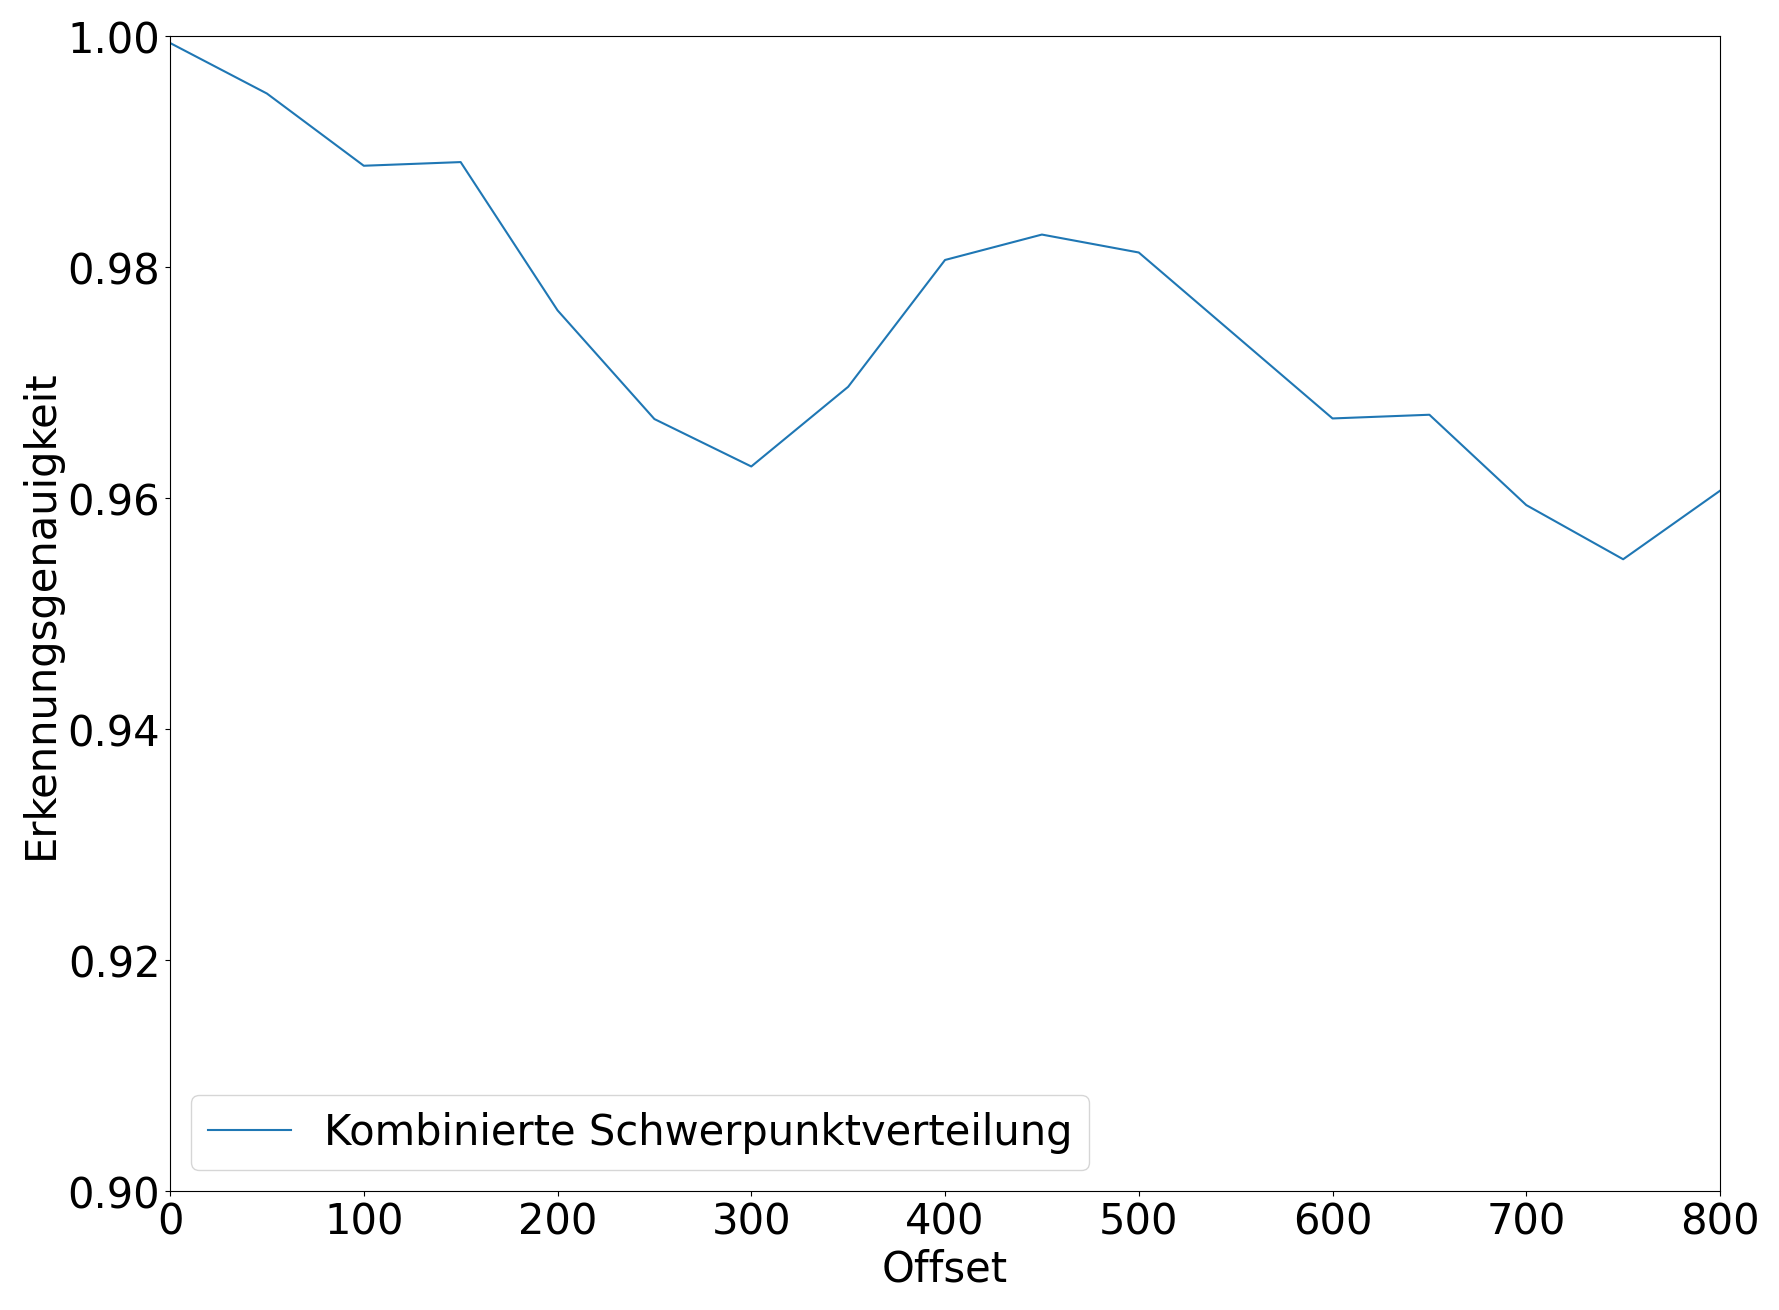
\includegraphics[width=0.495\linewidth]{images/brightness_offset_single.png}}\hfill%
\subfigure[Skalierung]{\label{subfig:brightness_cocd_comb_scaling}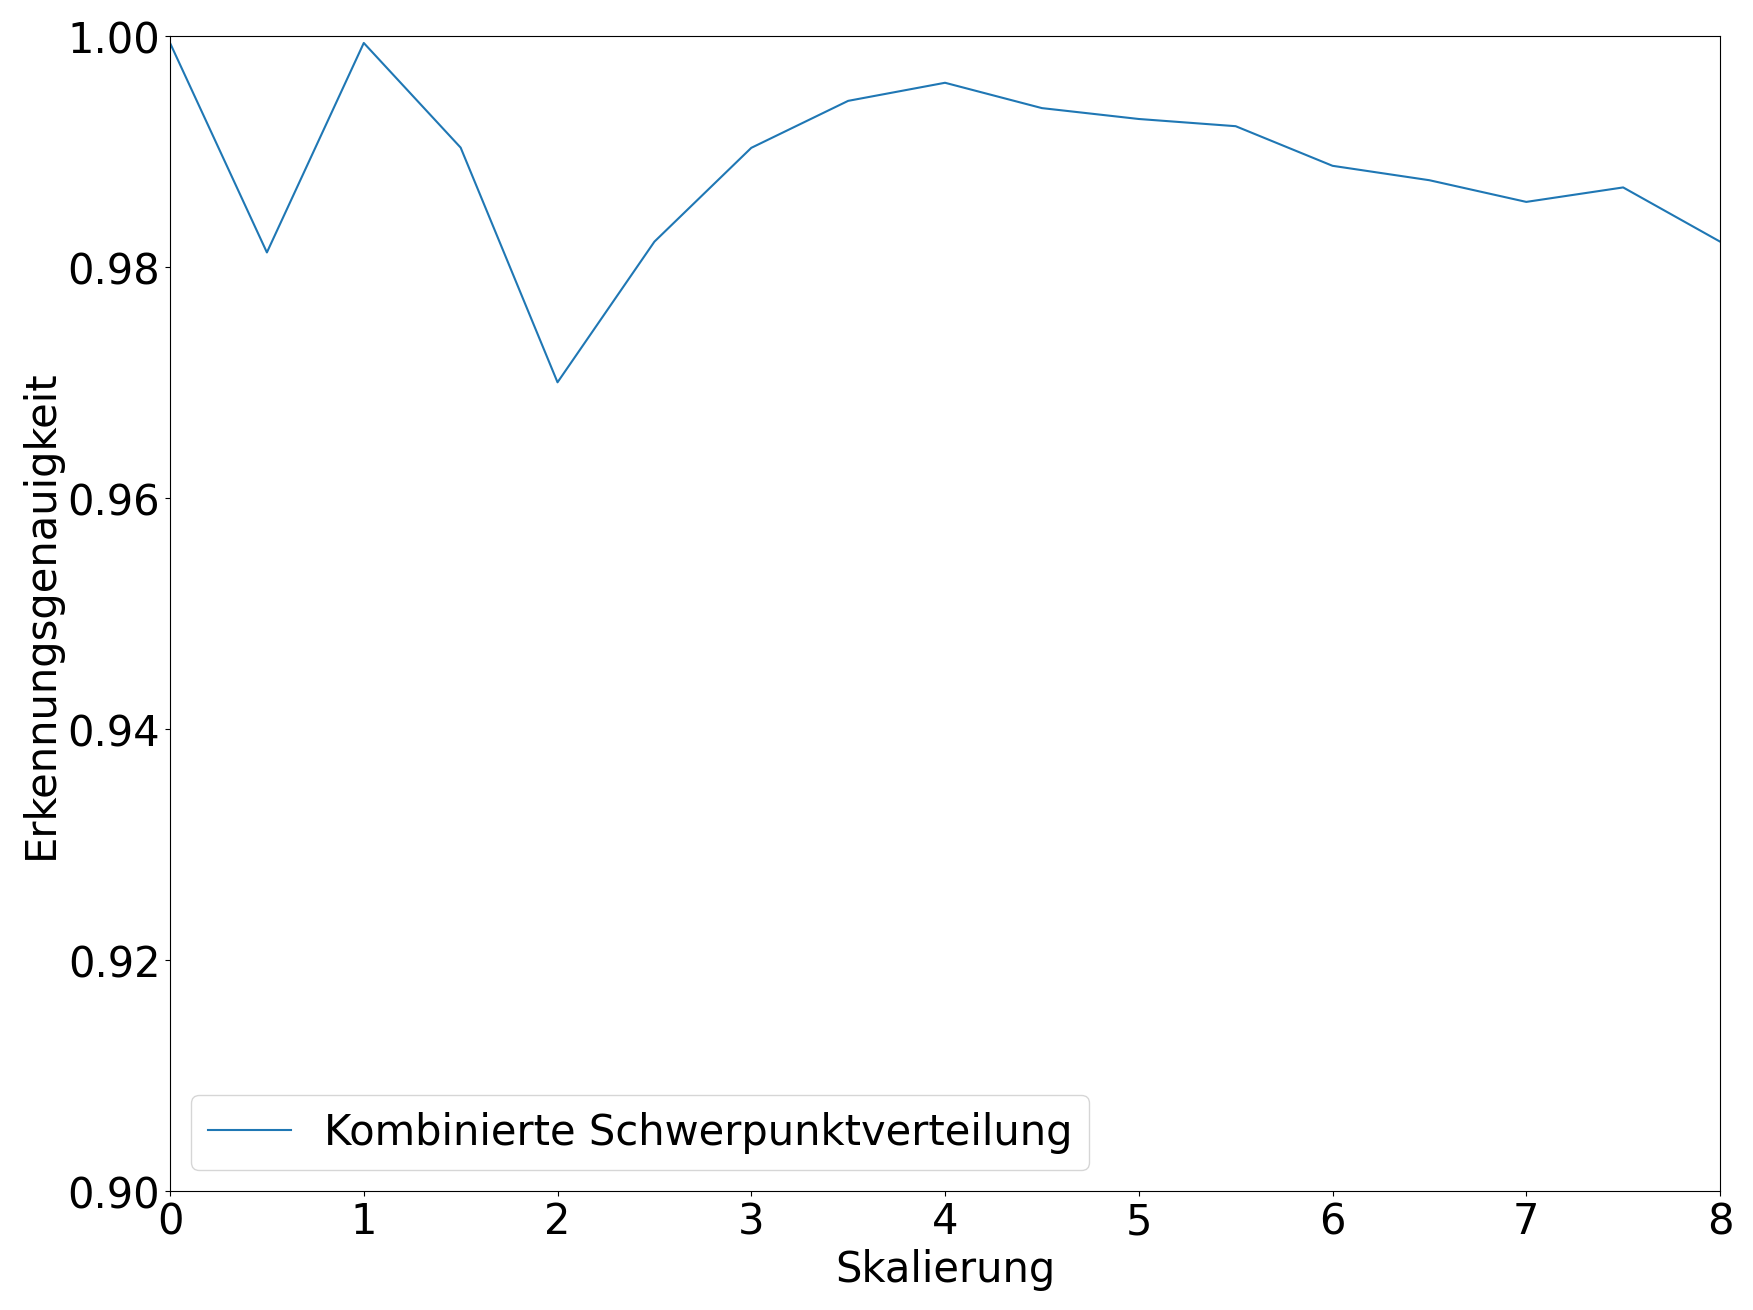
\includegraphics[width=0.495\linewidth]{images/brightness_scaling_single.png}}%
}{Ergebnisse der Testmenge für Lichtverhältnisse von dem kombinierten Klassifizierer.}{fig:brightness_cocd_comb}
\newline
\newline
Abbildung \ref{fig:brightness_cocd_comb} zeigt, dass der kombinierte Klassifizierer zwar nicht invariant gegenüber Skalierung und dem Offset ist, aber die Erkennungsgenauigkeit nimmt mit zunehmender
Skalierung bzw. Offset nur 2\% bis 4\% ab. Insgesamt ist die Erkennungsgenauigkeit der Testmenge für Lichtverhältnisse bei $98,1\%$.
\newline
\newline
Der Nachteil dieses Ansatzes ist, dass sowhl die Fearturmenge mit Gleitkommazahlen, als auch für Integer berechnet werden muss.
